\documentclass[12pt,a4paper]{article}
\usepackage[utf8]{inputenc}
\usepackage[margin=1in]{geometry}
\usepackage{graphicx}
\usepackage{amsmath}
\usepackage{hyperref}
\usepackage{listings}
\usepackage{xcolor}
\usepackage{booktabs}
\usepackage{float}
\usepackage{caption}

% Define colors for code listings
\definecolor{codegreen}{rgb}{0,0.6,0}
\definecolor{codegray}{rgb}{0.5,0.5,0.5}
\definecolor{codepurple}{rgb}{0.58,0,0.82}
\definecolor{backcolour}{rgb}{0.95,0.95,0.92}

% Configure code listings
\lstdefinestyle{mystyle}{
    backgroundcolor=\color{backcolour},   
    commentstyle=\color{codegreen},
    keywordstyle=\color{magenta},
    numberstyle=\tiny\color{codegray},
    stringstyle=\color{codepurple},
    basicstyle=\ttfamily\small,
    breakatwhitespace=false,         
    breaklines=true,                 
    captionpos=b,                    
    keepspaces=true,                 
    numbers=left,                    
    numbersep=5pt,                  
    showspaces=false,                
    showstringspaces=false,
    showtabs=false,                  
    tabsize=2
}
\lstset{style=mystyle}

\begin{document}

\begin{titlepage}
    \centering
    \vspace*{0.5cm}
    
    % Institution Logo
    
\includegraphics[width=0.3\textwidth]{kgp.jpeg}\par
    \vspace{1cm}
    
    % Institution Name
    {\LARGE \textbf{Indian Institute of Technology Kharagpur}}\par
    \vspace{0.8cm}
    % \newline
    % Project Title
    {\Huge \textbf{Query Processor and Optimizer}}\par
    \vspace{0.4cm}
    
    % Subtitle
    {\Large A Cost-Based Query Optimization System}\par
    \vspace{1.2cm}
    
    % Course Name and Instructors
    {\large \textbf{Course:} Database Management Systems (CS30202)}\par
    \vspace{0.3cm}
    {\large \textbf{Instructors:} Prof. Pabitra Mitra \& Prof. K.S. Rao}\par
    \vspace{1.5cm}
    
    % Group Members
    {\large \textbf{Group Members}}\par
    \vspace{0.5cm}
    \begin{tabular}{rl}
        \textbf{Name} & \textbf{Roll Number} \\
        \hline
        Dadi Sasank Kumar & 22CS10020 \\
        Jeevan Varma & 22CS10038 \\
        Gurram Dhanunjay & 22CS10029 \\
        Venkata Yaswanth & 22CS30031 \\
        Nerella Trilochan & 22CS10048 \\
    \end{tabular}
    
    \vfill
    
    % Submission Date
    {\large Submitted: April 15, 2025}\par
    \vspace{0.5cm}
    
    \rule{0.5\textwidth}{0.4pt}
\end{titlepage}

\tableofcontents


\newpage

\section{Problem Statement}
The objective of this project is to develop a query processor and optimizer for a relational database system. The system parses SQL SELECT queries, constructs an abstract syntax tree (AST), and optimizes the execution plan using selection pushdown and projection pushdown techniques. By leveraging table and column statistics, the optimizer estimates costs to select the most efficient plan, minimizing computational resources and execution time. The system supports SQL constructs such as SELECT, FROM, WHERE, JOIN, and aggregate functions (COUNT, MAX, MIN, AVG), providing detailed cost analyses for different execution plans.

This report includes a detailed analysis of the following SQL query:

\begin{lstlisting}[language=SQL]
SELECT employees.name, departments.dept_name 
FROM employees 
JOIN departments 
ON employees.dept_id = departments.dept_id 
WHERE departments.dept_name = 'Engineering';
\end{lstlisting}

The query leverage the available table and column statistics for cost-based optimization, constrained by the hardcoded metadata in \texttt{stats.cpp}/\texttt{stats.hpp}.

\section{Methodology}
The system is implemented in C++
, utilizing Flex for lexical analysis, Bison for parsing, and custom modules for optimization and statistics management. The processing pipeline consists of the following stages:

\subsection{Lexical Analysis}
The lexical analyzer (\texttt{lexer.l}) tokenizes SQL queries using Flex. It recognizes keywords (e.g., SELECT, FROM, WHERE, JOIN), identifiers, numbers, and operators in a case-insensitive manner. Debugging options enable token tracing for validation.

\subsection{Parsing}
The parser (\texttt{parser.y}), built with Bison, generates an AST from the tokenized query. Nodes represent operations (projection $\pi$, selection $\sigma$, join $\bowtie$), tables, conditions, and expressions. The parser handles column selections, table aliases, joins, conditions, and subqueries. The resulting AST, shown in Figure \ref{fig:original_ast}, captures the query’s logical structure.

\begin{figure}[H]
    \centering
    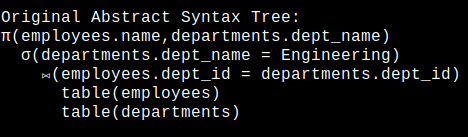
\includegraphics[width=0.8\textwidth]{original_ast.png}
    \caption{Original Abstract Syntax Tree}
    \label{fig:original_ast}
\end{figure}

\subsection{Statistics Management}
The statistics module (\texttt{stats.cpp}, \texttt{stats.hpp}) initializes hardcoded metadata for four tables: \texttt{employees}, \texttt{salaries}, \texttt{departments}, and \texttt{projects}. Each table includes row counts, column counts, and column statistics (distinct values, min/max values, selectivity). Functions like \texttt{calculate\_join\_selectivity} and \texttt{calculate\_condition\_selectivity} estimate the impact of joins and conditions, supporting cost-based optimization.

\subsection{Query Optimization}
The optimizer (\texttt{optimizer.cpp}, \texttt{optimizer.hpp}) applies two optimization techniques:
\begin{itemize}
    \item \textbf{Selection Pushdown}: Reorders selection operations ($\sigma$) closer to table scans to filter rows early, reducing intermediate result sizes.
    \item \textbf{Projection Pushdown}: Moves projection operations ($\pi$) toward table scans to limit column processing, minimizing data overhead.
\end{itemize}
The \texttt{estimate\_cost} function calculates result size, column count, and cost (rows $\times$ columns), while \texttt{calculate\_total\_plan\_cost} incorporates selectivity and column ratios. The optimizer evaluates multiple plans and selects the one with the lowest cost.

\subsection{Main Program}
The main program (\texttt{main.cpp}) reads a query from \texttt{query.sql}, parses it, optimizes the AST, and outputs execution plans with cost estimates. It integrates all modules to produce optimized query plans.

\subsection{Key Data Structures}
\begin{itemize}
    \item \textbf{Node} (\texttt{parser.hpp}): Represents AST nodes with fields for operation, arguments, child, and sibling pointers.
    \item \textbf{JoinOrderNode} (\texttt{optimizer.hpp}): Supports join order optimization (partially implemented).
    \item \textbf{CostMetrics} (\texttt{optimizer.hpp}): Stores result size, column count, and cost.
    \item \textbf{TableStats} and \textbf{ColumnStats} (\texttt{stats.hpp}): Hold table and column metadata.
\end{itemize}

\section{Results and Demonstration}
The system was tested with a sample query selecting \texttt{employees.name} and \texttt{departments.dept\_name} with a condition \texttt{departments.dept\_name = 'Engineering'} and a join on \texttt{employees.dept\_id = departments.dept\_id}. The results demonstrate parsing and optimization effectiveness across multiple stages.

\newpage
\subsection{Original Execution Plan}
The unoptimized execution plan, derived from the AST, includes all operations in their parsed order, with costs estimated using table statistics. The plan structure is as follows:

% \begin{verbatim}
% π(employees.name,departments.dept_name) [rows=500, cols=2, cost=1000.0]
%   σ(departments.dept_name = Engineering) [rows=500, cols=7, cost=3500.0]
%     ⨝(employees.dept_id = departments.dept_id) [rows=10000, cols=7, cost=70000.0]
%       table(employees) [rows=10000, cols=4, cost=40000.0]
%       table(departments) [rows=20, cols=3, cost=60.0]
% \end{verbatim}

% Figure \ref{fig:original_execplan} illustrates this plan.

\begin{figure}[H]
    \centering
    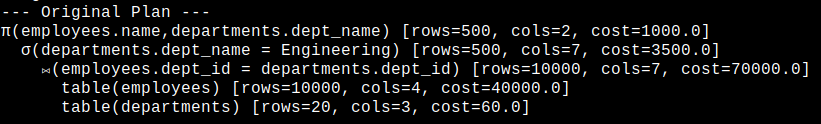
\includegraphics[width=0.8\textwidth]{original_execplan.png}
    \caption{Original Execution Plan}
    \label{fig:original_execplan}
\end{figure}

The cost breakup is detailed in Table \ref{tab:original_cost}.

\begin{table}[H]
    \centering
    \caption{Cost Breakup for Original Plan}
    \begin{tabular}{llcc}
        \toprule
        Node Type & Description & Node Cost & Cumulative Cost \\
        \midrule
        $\pi$ & employees.name,departments.dept\_name & 1000.0 & 45883.5 \\
        $\sigma$ & departments.dept\_name = Engineering & 3500.0 & 49413.0 \\
        $\bowtie$ & employees.dept\_id = departments.dept\_id & 70000.0 & 47060.0 \\
        table & employees & 40000.0 & 40000.0 \\
        table & departments & 60.0 & 60.0 \\
        \midrule
        Total & & & 45883.5 \\
        \bottomrule
    \end{tabular}
    \label{tab:original_cost}
\end{table}

\subsubsection{Cost Calculation for Original Plan}
The cumulative cost is computed bottom-up using \texttt{calculate\_total\_plan\_cost}:

\begin{itemize}
    \item \textbf{Table (employees)}:
        \begin{itemize}
            \item Node Cost: $10000 \times 4 = 40000.0$
            \item Cumulative Cost: For a table, returns \texttt{estimate\_cost.cost}.
            \item Formula: $\text{return current.cost}$
            \item Result: $40000.0$
        \end{itemize}
    \item \textbf{Table (departments)}:
        \begin{itemize}
            \item Node Cost: $20 \times 3 = 60.0$
            \item Cumulative Cost: $60.0$
            \item Formula: $\text{return current.cost}$
            \item Result: $60.0$
        \end{itemize}
    \item \textbf{Join ($\bowtie$)}:
        \begin{itemize}
            \item Node Cost: $10000 \times 7 = 70000.0$
            \item Selectivity: \texttt{get\_join\_selectivity} returns $0.05$ (default).
            \item Child Costs: Left (employees): $40000.0$, Right (departments): $60.0$
            \item Cumulative Cost:
                \begin{itemize}
                    \item Formula: $\text{left\_cost} + \text{right\_cost} + (\text{result\_size} \times \text{num\_columns} \times 0.1)$
                    \item Calculation: $40000.0 + 60.0 + (10000 \times 7 \times 0.1) = 40060.0 + 7000.0 = 47060.0$
                \end{itemize}
            \item Result: $47060.0$
        \end{itemize}
    \item \textbf{Selection ($\sigma$)}:
        \begin{itemize}
            \item Node Cost: $500 \times 7 = 3500.0$
            \item Selectivity: \texttt{get\_condition\_selectivity} returns $0.05$.
            \item Child Cost (join): $47060.0$
            \item Cumulative Cost:
                \begin{itemize}
                    \item Formula: $\text{child\_cost} \times (1.0 + \text{selectivity})$
                    \item Calculation: $47060.0 \times (1.0 + 0.05) = 47060.0 \times 1.05 = 49413.0$
                \end{itemize}
            \item Result: $49413.0$
        \end{itemize}
    \item \textbf{Projection ($\pi$)}:
        \begin{itemize}
            \item Node Cost: $500 \times 2 = 1000.0$
            \item Child Cost (selection): $49413.0$
            \item Column Ratio: $\text{num\_columns} / \text{child\_num\_columns} = 2 / 7 \approx 0.2857$
            \item Cumulative Cost:
                \begin{itemize}
                    \item Formula: $\text{child\_cost} \times (0.9 + 0.1 \times \text{column\_ratio})$
                    \item Calculation: $49413.0 \times (0.9 + 0.1 \times 0.2857) = 49413.0 \times (0.9 + 0.02857) \approx 49413.0 \times 0.92857 \approx 45883.5$
                \end{itemize}
            \item Result: $45883.5$
        \end{itemize}
\end{itemize}

The total cost is the cumulative cost of the root node ($\pi$): $45883.5$. Node costs ($1000.0 + 3500.0 + 70000.0 + 40000.0 + 60.0 = 114560.0$) don’t sum to the total because cumulative costs incorporate selectivity ($1.05$ for $\sigma$, $0.05$ for $\bowtie$) and column ratio ($0.2857$ for $\pi$), reflecting filtering and projection efficiencies. The table shows subtree costs, with the root’s cost as the total plan cost.
\newpage
\subsection{Selection Pushdown Optimization}
Selection pushdown reorders the selection to filter \texttt{departments} before the join, reducing the join’s input size. The plan structure is:

% \begin{verbatim}
% π(employees.name,departments.dept_name) [rows=500, cols=2, cost=1000.0]
%   ⨝(employees.dept_id = departments.dept_id) [rows=500, cols=7, cost=3500.0]
%     table(employees) [rows=10000, cols=4, cost=40000.0]
%     σ(departments.dept_name = Engineering) [rows=1, cols=3, cost=3.0]
%       table(departments) [rows=20, cols=3, cost=60.0]
% \end{verbatim}

Figure \ref{fig:selection_pushdown_exceplan} illustrates this plan.

\begin{figure}[H]
    \centering
    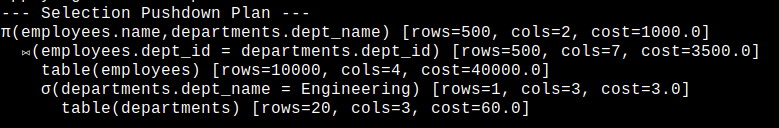
\includegraphics[width=0.8\textwidth]{selection_pushdown_exceplan.png}
    \caption{Selection Pushdown Execution Plan}
    \label{fig:selection_pushdown_exceplan}
\end{figure}

The cost breakup is provided in Table \ref{tab:selection_cost}.

\begin{table}[H]
    \centering
    \caption{Cost Breakup for Selection Pushdown Plan}
    \begin{tabular}{llcc}
        \toprule
        Node Type & Description & Node Cost & Cumulative Cost \\
        \midrule
        $\pi$ & employees.name,departments.dept\_name & 1000.0 & 37526.4 \\
        $\bowtie$ & employees.dept\_id = departments.dept\_id & 3500.0 & 40413.0 \\
        table & employees & 40000.0 & 40000.0 \\
        $\sigma$ & departments.dept\_name = Engineering & 3.0 & 63.0 \\
        table & departments & 60.0 & 60.0 \\
        \midrule
        Total & & & 37526.4 \\
        \bottomrule
    \end{tabular}
    \label{tab:selection_cost}
\end{table}

\subsubsection{Cost Calculation for Selection Pushdown Plan}
The cumulative cost is computed bottom-up:

\begin{itemize}
    \item \textbf{Table (departments)}:
        \begin{itemize}
            \item Node Cost: $20 \times 3 = 60.0$
            \item Cumulative Cost: $60.0$
            \item Formula: $\text{return current.cost}$
            \item Result: $60.0$
        \end{itemize}
    \item \textbf{Selection ($\sigma$)}:
        \begin{itemize}
            \item Node Cost: $1 \times 3 = 3.0$
            \item Selectivity: $0.05$
            \item Child Cost (departments): $60.0$
            \item Cumulative Cost:
                \begin{itemize}
                    \item Formula: $\text{child\_cost} \times (1.0 + \text{selectivity})$
                    \item Calculation: $60.0 \times (1.0 + 0.05) = 60.0 \times 1.05 = 63.0$
                \end{itemize}
            \item Result: $63.0$
        \end{itemize}
        \newpage
    \item \textbf{Table (employees)}:
        \begin{itemize}
            \item Node Cost: $10000 \times 4 = 40000.0$
            \item Cumulative Cost: $40000.0$
            \item Formula: $\text{return current.cost}$
            \item Result: $40000.0$
        \end{itemize}
    \item \textbf{Join ($\bowtie$)}:
        \begin{itemize}
            \item Node Cost: $500 \times 7 = 3500.0$
            \item Selectivity: $0.05$
            \item Child Costs: Left (employees): $40000.0$, Right ($\sigma$): $63.0$
            \item Cumulative Cost:
                \begin{itemize}
                    \item Formula: $\text{left\_cost} + \text{right\_cost} + (\text{result\_size} \times \text{num\_columns} \times 0.1)$
                    \item Calculation: $40000.0 + 63.0 + (500 \times 7 \times 0.1) = 40063.0 + 350.0 = 40413.0$
                \end{itemize}
            \item Result: $40413.0$
        \end{itemize}
    \item \textbf{Projection ($\pi$)}:
        \begin{itemize}
            \item Node Cost: $500 \times 2 = 1000.0$
            \item Child Cost (join): $40413.0$
            \item Column Ratio: $2 / 7 \approx 0.2857$
            \item Cumulative Cost:
                \begin{itemize}
                    \item Formula: $\text{child\_cost} \times (0.9 + 0.1 \times \text{column\_ratio})$
                    \item Calculation: $40413.0 \times (0.9 + 0.1 \times 0.2857) = 40413.0 \times (0.9 + 0.02857) \approx 40413.0 \times 0.92857 \approx 37526.4$
                \end{itemize}
            \item Result: $37526.4$
        \end{itemize}
\end{itemize}

The total cost is $37526.4$. The selection reduces \texttt{departments} to 1 row before the join, lowering the join’s result to 500 rows (vs. 10000), reducing the cost (40413.0 vs. 47060.0). Node costs ($1000.0 + 3500.0 + 40000.0 + 3.0 + 60.0 = 44563.0$) don’t sum to the total due to selectivity ($1.05$ for $\sigma$, $0.05$ for $\bowtie$) and column ratio ($0.2857$ for $\pi$). The table reflects subtree costs, with the root’s cost as the total.
\newpage
\subsection{Projection Pushdown Optimization}
Projection pushdown applies projections early to reduce columns before the join and selection. The plan structure is:

% \begin{verbatim}
% σ(departments.dept_name = Engineering) [rows=500, cols=2, cost=1000.0]
%   π(employees.name,departments.dept_name) [rows=10000, cols=2, cost=20000.0]
%     ⨝(employees.dept_id = departments.dept_id) [rows=10000, cols=2, cost=20000.0]
%       π(employees.name,employees.dept_id) [rows=10000, cols=2, cost=20000.0]
%         table(employees) [rows=10000, cols=4, cost=40000.0]
%       π(departments.dept_name,departments.dept_id) [rows=20, cols=2, cost=40.0]
%         table(departments) [rows=20, cols=3, cost=60.0]
% \end{verbatim}

% Figure \ref{fig:projection_pushdown_execplan} illustrates this plan.

\begin{figure}[H]
    \centering
    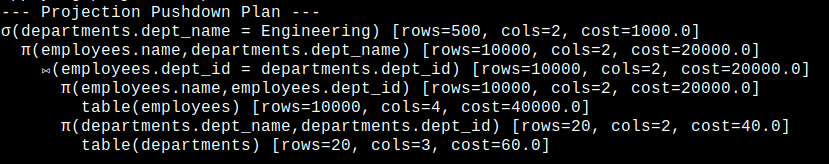
\includegraphics[width=0.8\textwidth]{projection_pushdown_execplan.png}
    \caption{Projection Pushdown Execution Plan}
    \label{fig:projection_pushdown_execplan}
\end{figure}

The cost breakup is detailed in Table \ref{tab:projection_cost}.

\begin{table}[H]
    \centering
    \caption{Cost Breakup for Projection Pushdown Plan}
    \begin{tabular}{llcc}
        \toprule
        Node Type & Description & Node Cost & Cumulative Cost \\
        \midrule
        $\sigma$ & departments.dept\_name = Engineering & 1000.0 & 42060.9 \\
        $\pi$ & employees.name,departments.dept\_name & 20000.0 & 40058.0 \\
        $\bowtie$ & employees.dept\_id = departments.dept\_id & 20000.0 & 40058.0 \\
        $\pi$ & employees.name,employees.dept\_id & 20000.0 & 38000.0 \\
        table & employees & 40000.0 & 40000.0 \\
        $\pi$ & departments.dept\_name,departments.dept\_id & 40.0 & 58.0 \\
        table & departments & 60.0 & 60.0 \\
        \midrule
        Total & & & 42060.9 \\
        \bottomrule
    \end{tabular}
    \label{tab:projection_cost}
\end{table}

\subsubsection{Cost Calculation for Projection Pushdown Plan}
The cumulative cost is computed bottom-up:

\begin{itemize}
    \item \textbf{Table (departments)}:
        \begin{itemize}
            \item Node Cost: $20 \times 3 = 60.0$
            \item Cumulative Cost: $60.0$
            \item Formula: $\text{return current.cost}$
            \item Result: $60.0$
        \end{itemize}
    \item \textbf{Projection ($\pi$, departments.dept\_name,departments.dept\_id)}:
        \begin{itemize}
            \item Node Cost: $20 \times 2 = 40.0$
            \item Child Cost (departments): $60.0$
            \item Column Ratio: $2 / 3 \approx 0.6667$
            \item Cumulative Cost:
                \begin{itemize}
                    \item Formula: $\text{child\_cost} \times (0.9 + 0.1 \times \text{column\_ratio})$
                    \item Calculation: $60.0 \times (0.9 + 0.1 \times 0.6667) = 60.0 \times (0.9 + 0.06667) \approx 60.0 \times 0.96667 \approx 58.0$
                \end{itemize}
            \item Result: $58.0$
        \end{itemize}
    \item \textbf{Table (employees)}:
        \begin{itemize}
            \item Node Cost: $10000 \times 4 = 40000.0$
            \item Cumulative Cost: $40000.0$
            \item Formula: $\text{return current.cost}$
            \item Result: $40000.0$
        \end{itemize}
    \item \textbf{Projection ($\pi$, employees.name,employees.dept\_id)}:
        \begin{itemize}
            \item Node Cost: $10000 \times 2 = 20000.0$
            \item Child Cost (employees): $40000.0$
            \item Column Ratio: $2 / 4 = 0.5$
            \item Cumulative Cost:
                \begin{itemize}
                    \item Formula: $\text{child\_cost} \times (0.9 + 0.1 \times \text{column\_ratio})$
                    \item Calculation: $40000.0 \times (0.9 + 0.1 \times 0.5) = 40000.0 \times (0.9 + 0.05) = 40000.0 \times 0.95 = 38000.0$
                \end{itemize}
            \item Result: $38000.0$
        \end{itemize}
        % \newpage
    \item \textbf{Join ($\bowtie$)}:
        \begin{itemize}
            \item Node Cost: $10000 \times 2 = 20000.0$
            \item Selectivity: $0.05$
            \item Child Costs: Left ($\pi$ employees): $38000.0$, Right ($\pi$ departments): $58.0$
            \item Cumulative Cost:
                \begin{itemize}
                    \item Formula: $\text{left\_cost} + \text{right\_cost} + (\text{result\_size} \times \text{num\_columns} \times 0.1)$
                    \item Calculation: $38000.0 + 58.0 + (10000 \times 2 \times 0.1) = 38058.0 + 2000.0 = 40058.0$
                \end{itemize}
            \item Result: $40058.0$
        \end{itemize}
    \item \textbf{Projection ($\pi$, employees.name,departments.dept\_name)}:
        \begin{itemize}
            \item Node Cost: $10000 \times 2 = 20000.0$
            \item Child Cost (join): $40058.0$
            \item Column Ratio: $2 / 2 = 1.0$
            \item Cumulative Cost:
                \begin{itemize}
                    \item Formula: $\text{child\_cost} \times (0.9 + 0.1 \times \text{column\_ratio})$
                    \item Calculation: $40058.0 \times (0.9 + 0.1 \times 1.0) = 40058.0 \times (0.9 + 0.1) = 40058.0 \times 1.0 = 40058.0$
                \end{itemize}
            \item Result: $40058.0$
        \end{itemize}
    \item \textbf{Selection ($\sigma$)}:
        \begin{itemize}
            \item Node Cost: $500 \times 2 = 1000.0$
            \item Selectivity: $0.05$
            \item Child Cost ($\pi$): $40058.0$
            \item Cumulative Cost:
                \begin{itemize}
                    \item Formula: $\text{child\_cost} \times (1.0 + \text{selectivity})$
                    \item Calculation: $40058.0 \times (1.0 + 0.05) = 40058.0 \times 1.05 \approx 42060.9$
                \end{itemize}
            \item Result: $42060.9$
        \end{itemize}
\end{itemize}

The total cost is $42060.9$. Projections reduce columns early (2 vs. 7 in join), but the join processes 10000 rows since selection is applied last. Node costs ($1000.0 + 20000.0 + 20000.0 + 20000.0 + 40000.0 + 40.0 + 60.0 = 101000.0$) don’t sum to the total due to column ratio reductions ($0.95$, $0.96667$) and selectivity ($0.05$). The table shows subtree costs, with the root’s cost as the total.

\subsection{Cost Comparison}
The optimizer compares the three plans based on total cost, result size, and column count. The comparison is visualized in Figure \ref{fig:cost_comparison} and summarized in Table \ref{tab:cost_comparison}.

\begin{figure}[H]
    \centering
    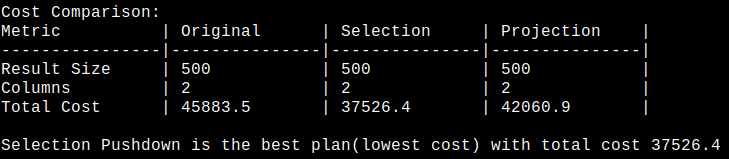
\includegraphics[width=0.8\textwidth]{cost_comparison.png}
    \caption{Cost Comparison of Execution Plans}
    \label{fig:cost_comparison}
\end{figure}

\begin{table}[H]
    \centering
    \caption{Cost Comparison Across Plans}
    \begin{tabular}{lccc}
        \toprule
        Metric & Original & Selection Pushdown & Projection Pushdown \\
        \midrule
        Result Size & 500 & 500 & 500 \\
        Columns & 2 & 2 & 2 \\
        Total Cost & 45883.5 & 37526.4 & 42060.9 \\
        \bottomrule
    \end{tabular}
    \label{tab:cost_comparison}
\end{table}

The selection pushdown plan is the most efficient because it reduces the join’s input size to 1 row for \texttt{departments}, yielding a join result of 500 rows, lowering the cost to 37526.4. The original plan (45883.5) processes 10000 rows in the join, while projection pushdown (42060.9) reduces columns but not rows until the final selection.
\newpage
\section{Conclusion and Future Scope}
The query processor and optimizer successfully parse SQL queries, generate ASTs, and produce optimized execution plans. The selection pushdown plan achieves the lowest cost (37526.4), as shown in Table \ref{tab:selection_cost}, by filtering rows early. Projection pushdown reduces column overhead but incurs a higher cost (42060.9) due to processing 10000 rows in the join, as seen in Table \ref{tab:projection_cost}. The original plan is the least efficient (45883.5), confirming the value of optimization.

\subsection{Future Scope}
\begin{itemize}
    \item \textbf{Join Reordering}: Implement \texttt{reorder\_joins} and \texttt{find\_optimal\_join\_order} to optimize join sequences.
    \item \textbf{Dynamic Statistics}: Replace hardcoded statistics with metadata file updates.
    \item \textbf{Subquery Optimization}: Enhance support for nested and correlated subqueries.
    \item \textbf{Parallel Execution}: Introduce parallel processing for joins and selections.
    
\end{itemize}

\section{References}
\begin{enumerate}
    \item Silberschatz, A., Korth, H. F., \& Sudarshan, S. (2019). \textit{Database System Concepts} (7th ed.). McGraw-Hill Education.
    \item Flex \& Bison documentation: \url{https://www.gnu.org/software/flex/}, \url{https://www.gnu.org/software/bison/}
    \item Ramakrishnan, R., \& Gehrke, J. (2002). \textit{Database Management Systems} (3rd ed.). McGraw-Hill Education.
\end{enumerate}

\end{document}